\documentclass[tikz,border=3pt]{standalone}
\usepackage{fontspec}
\usepackage{amsmath}
\usepackage{xcolor}
\usepackage{tikz}
\usepackage{pgfplots}
\pgfplotsset{compat=1.18}
\usetikzlibrary{arrows.meta,calc,fit,positioning,shapes.geometric,shapes.misc,patterns,plotmarks}
\IfFontExistsTF{Arial}{\setsansfont{Arial}}{\setsansfont{TeX Gyre Heros}}
\renewcommand{\familydefault}{\sfdefault}
\tikzset{
  >={Stealth[length=2.2mm,width=1.5mm]},
  exact title/.style={font=\bfseries\fontsize{10.5}{12}\selectfont,align=center},
  exact subtitle/.style={font=\fontsize{6.3}{7.2}\selectfont,align=center},
  exact label/.style={font=\fontsize{6.4}{7.5}\selectfont,align=center},
  exact tiny/.style={font=\fontsize{5.3}{6.3}\selectfont,align=center},
  panel/.style={draw=black!14,rounded corners=1.2mm,fill=white,line width=.45pt},
  neutral/.style={draw=black!30,fill=black!3,rounded corners=1mm,line width=.45pt},
  arrow/.style={-Stealth,line width=.7pt},
  softarrow/.style={-Stealth,line width=.55pt,draw=black!45},
  dashedarrow/.style={-Stealth,dashed,line width=.55pt,draw=black!55},
  metric/.style={font=\fontsize{5.3}{6.3}\selectfont,fill=white,inner sep=1pt},
}
\newcommand{\pill}[4]{\node[draw=#2!70,fill=#2!10,rounded corners=1.5mm,inner xsep=3pt,inner ysep=2pt,exact label,text=#2] (#1) at #3 {#4};}
\newcommand{\frameboxx}[4]{\draw[draw=#2!65,fill=#2!8,rounded corners=.6mm,line width=.5pt] (#1.south west) rectangle (#1.north east);\node[exact tiny,text=#2] at #3 {#4};}
\newcommand{\axislabel}[3]{\node[exact tiny,text=black!60] at (#1) {#2};\node[exact tiny,text=black!60,rotate=90] at (#3) {#2};}

\definecolor{spred}{HTML}{ED1C24}\definecolor{spyellow}{HTML}{FFDE17}\definecolor{sppurple}{HTML}{7F3F98}\definecolor{spgreen}{HTML}{2CA02C}\definecolor{spblue}{HTML}{1F77B4}\definecolor{sporange}{HTML}{FF7F0E}\definecolor{spink}{HTML}{263238}
\begin{document}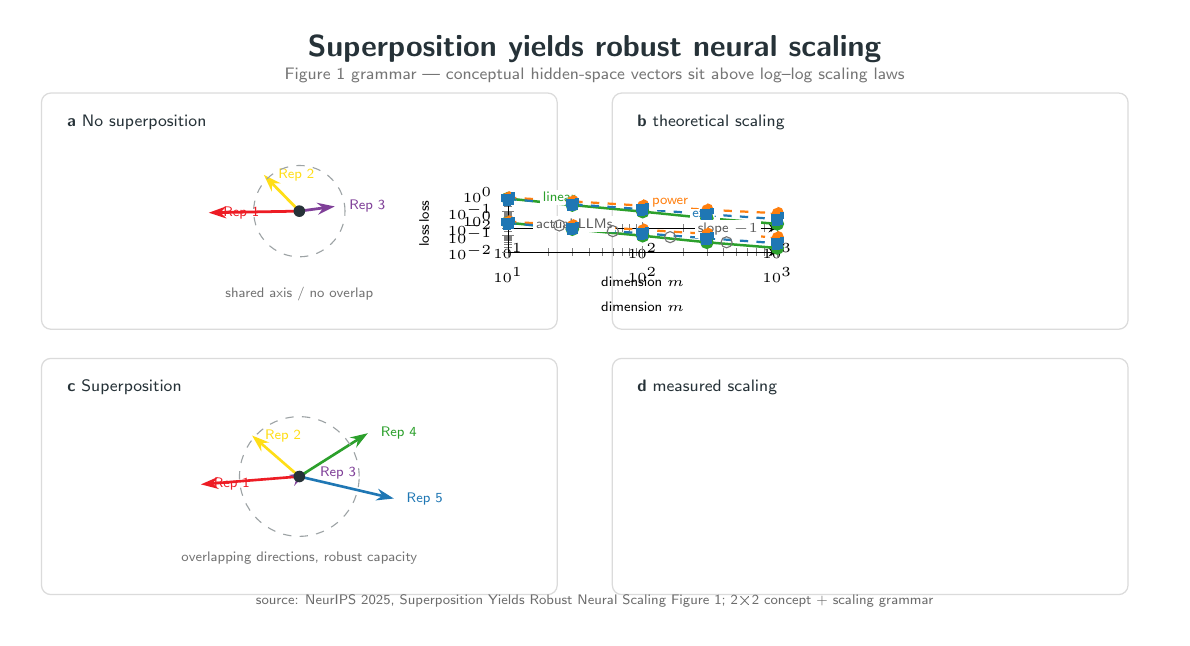
\begin{tikzpicture}[x=1cm,y=1cm]
\path[use as bounding box] (-.2,-5.05) rectangle (14.2,2.45);
\node[exact title,text=spink] at (7,2.18) {Superposition yields robust neural scaling};
\node[exact subtitle,text=black!54] at (7,1.84) {Figure 1 grammar — conceptual hidden-space vectors sit above log–log scaling laws};
\node[panel,minimum width=6.55cm,minimum height=3.0cm] (a) at (3.25,.12) {};
\node[panel,minimum width=6.55cm,minimum height=3.0cm] (b) at (10.5,.12) {};
\node[panel,minimum width=6.55cm,minimum height=3.0cm] (c) at (3.25,-3.25) {};
\node[panel,minimum width=6.55cm,minimum height=3.0cm] (d) at (10.5,-3.25) {};
\node[exact label,anchor=west,text=spink] at (0.18,1.25) {\textbf{a}  No superposition};
\node[exact label,anchor=west,text=spink] at (7.42,1.25) {\textbf{b}  theoretical scaling};
\node[exact label,anchor=west,text=spink] at (0.18,-2.12) {\textbf{c}  Superposition};
\node[exact label,anchor=west,text=spink] at (7.42,-2.12) {\textbf{d}  measured scaling};
\foreach \x/\y/\c/\lab in {2.1/.1/spred/Rep 1,2.8/.58/spyellow/Rep 2,3.7/.18/sppurple/Rep 3}{\draw[->,\c,line width=1pt] (3.25,.12) -- (\x,\y);\node[exact tiny,text=\c,anchor=west] at (\x+.06,\y) {\lab};}\fill[spink] (3.25,.12) circle (2.1pt);\draw[spink!45,dashed] (3.25,.12) circle (.58cm);\node[exact tiny,text=black!55] at (3.25,-.93) {shared axis / no overlap};
\foreach \x/\y/\c/\lab in {2.0/-.1/spred/Rep 1,2.65/.52/spyellow/Rep 2,3.35/.05/sppurple/Rep 3,4.12/.55/spgreen/Rep 4,4.45/-.28/spblue/Rep 5}{\draw[->,\c,line width=.95pt] (3.25,-3.25) -- (\x,\y-3.25);\node[exact tiny,text=\c,anchor=west] at (\x+.04,\y-3.25) {\lab};}\fill[spink] (3.25,-3.25) circle (2.1pt);\draw[spink!45,dashed] (3.25,-3.25) circle (.76cm);\node[exact tiny,text=black!55] at (3.25,-4.28) {overlapping directions, robust capacity};
\begin{axis}[at={(7.95,-1.05)},width=5.0cm,height=2.0cm,xmode=log,ymode=log,xmin=10,xmax=1000,ymin=.01,ymax=1,axis lines=left,xtick={10,100,1000},ytick={.01,.1,1},tick label style={font=\fontsize{4.5}{5}\selectfont},label style={font=\fontsize{4.8}{5}\selectfont},xlabel={dimension \(m\)},ylabel={loss},clip=false]
\addplot[spgreen,line width=.9pt,mark=*] coordinates {(10,.62)(30,.25)(100,.1)(300,.04)(1000,.018)};\addplot[sporange,dashed,line width=.8pt,mark=*] coordinates {(10,.72)(30,.42)(100,.23)(300,.13)(1000,.08)};\addplot[spblue,dashed,line width=.8pt,mark=square*] coordinates {(10,.58)(30,.28)(100,.14)(300,.07)(1000,.035)};\node[metric,text=spgreen] at (axis cs:24,.76) {linear};\node[metric,text=sporange] at (axis cs:160,.36) {power};\node[metric,text=spblue] at (axis cs:290,.055) {exp.};\end{axis}
\begin{axis}[at={(7.95,-4.42)},width=5.0cm,height=2.0cm,xmode=log,ymode=log,xmin=10,xmax=1000,ymin=.01,ymax=1,axis lines=left,xtick={10,100,1000},ytick={.01,.1,1},tick label style={font=\fontsize{4.5}{5}\selectfont},label style={font=\fontsize{4.8}{5}\selectfont},xlabel={dimension \(m\)},ylabel={loss},clip=false]
\addplot[spgreen,line width=.9pt,mark=*] coordinates {(10,.62)(30,.25)(100,.1)(300,.04)(1000,.018)};\addplot[sporange,dashed,line width=.8pt,mark=*] coordinates {(10,.72)(30,.42)(100,.23)(300,.13)(1000,.08)};\addplot[spblue,dashed,line width=.8pt,mark=square*] coordinates {(10,.58)(30,.28)(100,.14)(300,.07)(1000,.035)};\addplot[black!55,mark=o,only marks] coordinates {(24,.42)(60,.19)(160,.082)(420,.04)};\node[metric,text=black!65] at (axis cs:31,.52) {actual LLMs};\draw[black!60,-Stealth] (axis cs:260,.34) -- (axis cs:470,.12);\node[metric,text=black!65] at (axis cs:430,.27) {slope \(-1\)};\end{axis}
\node[exact tiny,text=black!58] at (7,-4.83) {source: NeurIPS 2025, Superposition Yields Robust Neural Scaling Figure 1; 2×2 concept + scaling grammar};
\end{tikzpicture}\end{document}
